\chapter{Experiments on MNIST}

\section{MNIST}

Jest to zbiór po kategoryzowanych odręcznie napisanych cyfr. Wszystkie obrazki są czarno-białe, rozmiaru 28x28 i wycentrowane. Zbiór składa się z 60000 danych treningowych i 10000 testowych. Zbiór ten często wykorzystywany jest w celach testowych. W sensie, że jeżeli model na nim nie zadziała, to z dużym prawdopodobieństwem nie zadziała również na bardziej skomplikowanych danych. Przykładowe obrazki \ref{fig:mnist}.

\begin{figure}[h!]
    \centering
    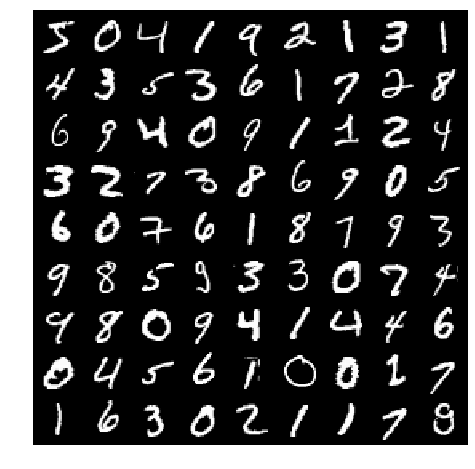
\includegraphics[width=0.4\textwidth]{images/mnist}
    \caption{Samples from MNIST dataset}
    \label{fig:mnist}
\end{figure}

\section{VAE}

Na rysunku \ref{fig:vae} znajduje się efekt wyuczenia modelu VAE z warstwą ukrytą rozmiaru 20. Po lewej widać rekonstrukcje, a po prawej efekty zdekodowania wektora wygenerowanego ze standardowego rozkładu normalnego.

\begin{figure}[h!]
  \centering
  \begin{subfigure}[b]{0.57\linewidth}
    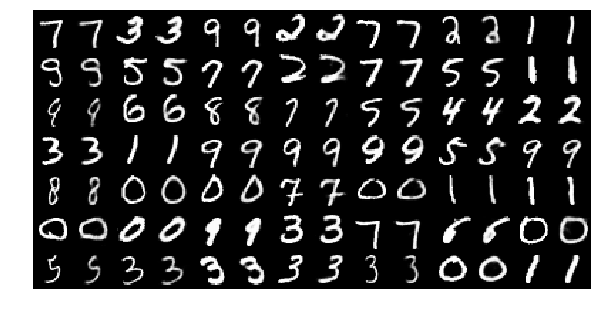
\includegraphics[width=\linewidth]{images/mnist_recon}
    \caption{Coffee.}
  \end{subfigure}
  \begin{subfigure}[b]{0.30\linewidth}
    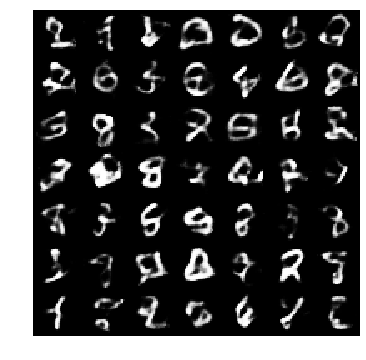
\includegraphics[width=\linewidth]{images/mnist_gen}
    \caption{More coffee.}
  \end{subfigure}
  \caption{The same cup of coffee. Two times.}
  \label{fig:vae}
\end{figure}
\todo{Uzupełnić podpisy}

Dodatkowo warto byłby zobaczyć jak konkretne cyfry rozrzucane są w przestrzeni. 20 wymiarów jest dosyć trudne do zwizualizowania, więc wyuczyłem model dla reprezentacji ukrytej rozmiaru 2. Na rysunku \ref{fig:mnist_2d} znajdują sie wyniki. Wartym odnotowania jest fakt, że niektóre klasy są bardzo dobrze separowalne, mimo iz podczas nauki nie staraliśmy się rozwiązywać problemu klasyfikacji. Te ciekawą własność wyniku reprezentacji będę chciał wykorzystać w późniejszej analizie.

\begin{figure}[h!]
    \centering
    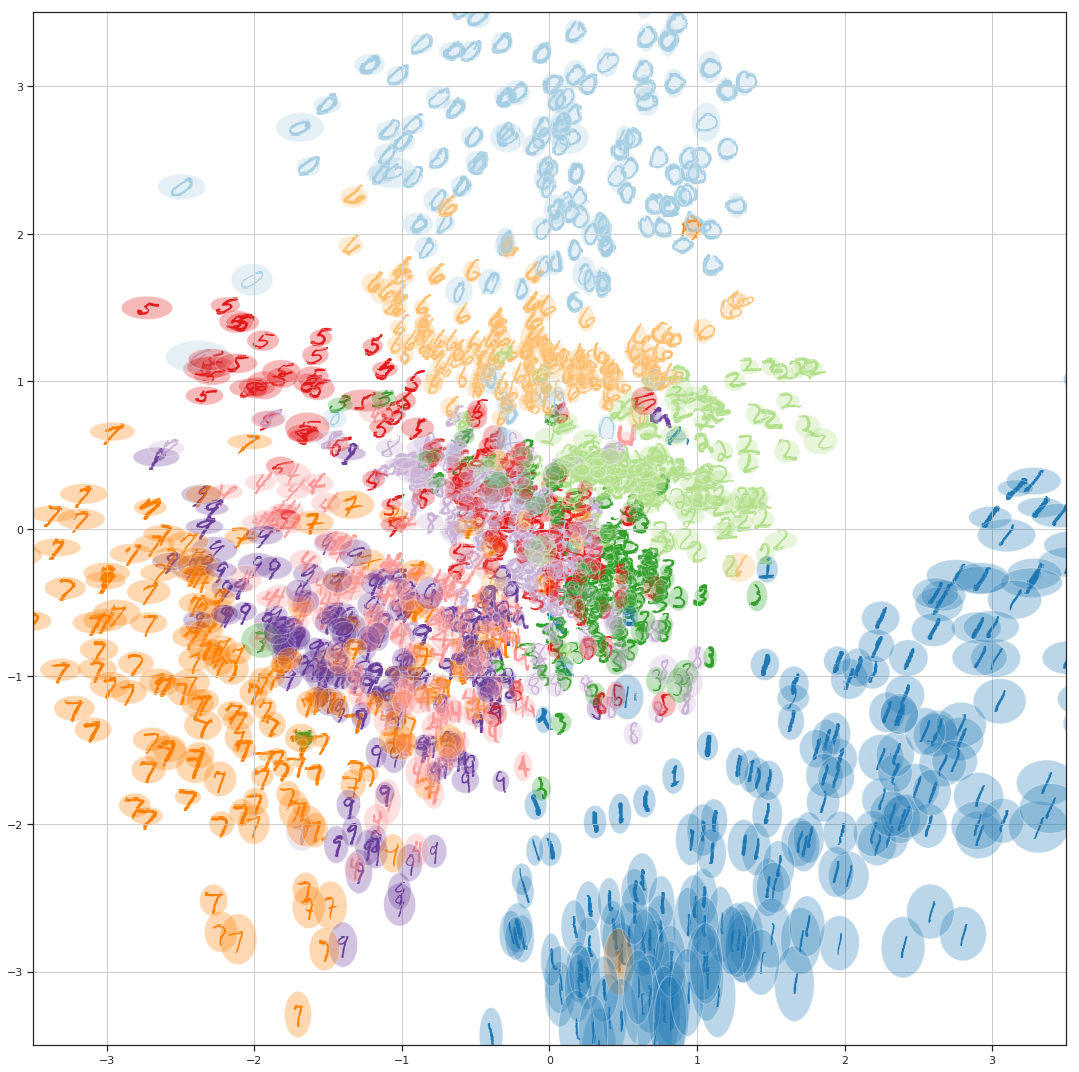
\includegraphics[width=1.\textwidth]{images/mnist_2d}
    \caption{}
    \label{fig:mnist_2d}
\end{figure}

W oryginalnym problemie mamy bardzo duży dysonans pomiędzy ilością przykładów dla każdej z klas. Według statystyk dane z komórkami rakowymi stanowią ~2\% wszystkich \todo{Do sprawdzenia}. Ciężko jest wiec nawet mówić o jakimś sensownym podejściu supervised. Do zasymulowania tego problemu dla MNIST będę uczył model jedynie na dwóch klasach [4, 7], a następnie testował zachowanie reprezentacji ukrytej dla przekładów z klasy 5.

Rozmiar reprezentacji ukrytej wynosi 10. Analizować natomiast będziemy 2 składowe kosztu dla modelu VAE: KLD oraz błąd rekonsrukcji MSE \todo{Opisać gdzieś te koszty}. Na rysunku \ref{fig:mnist_compare} znajduje się przedstawienie ich wraz z histogramami. Można zauważyć, że wyłącznie na podstawie samego błędu rekonstrukcji można z bardzo dużą dokładnością określić dane pochodzące z klasy 5, mimo iż model nie widział żadnych ich przykładów podczas uczenia.

\begin{figure}[h!]
    \centering
    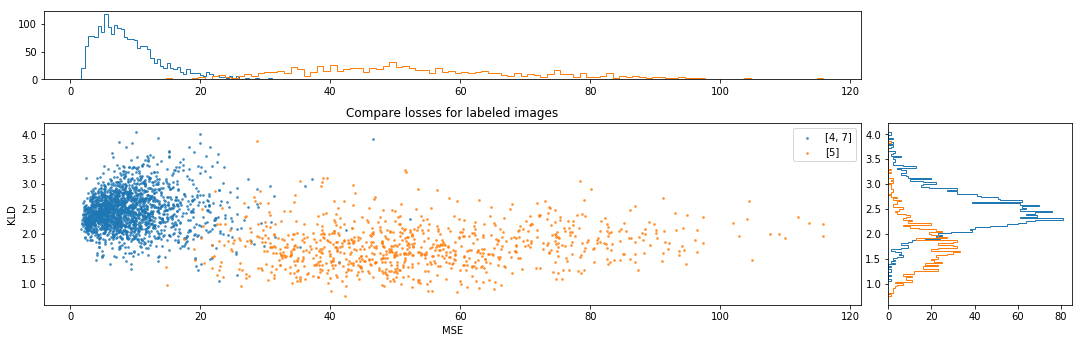
\includegraphics[width=1.0\textwidth]{images/mnist_compare}
    \caption{}
    \label{fig:mnist_compare}
\end{figure}

Do określenia jak rzeczywiście dobra jest ta separacja można wykorzystać krzywą ROC. Traktujemy to jako problem binarnej klasyfikacji, gdzie dane z klasy 5 będą oznaczone jako 1, a z [4, 7] jako 0. Wartość confidence to suma kosztów KLD i MSE. Jak widać na rysunku \ref{fig:mnist_roc} takie podejście osiąga prawie 100\% skuteczność. Podobne podejście będę chciał zastosować do danych medycznych.

\subsection{ROC}

Opis ROC

\begin{figure}[h!]
    \centering
    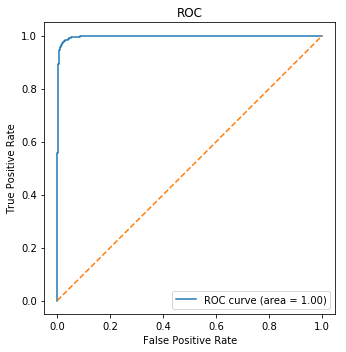
\includegraphics[width=0.5\textwidth]{images/mnist_roc}
    \caption{}
    \label{fig:mnist_roc}
\end{figure}

\section{Deep feature consistent variational auto-encoder}

Podobny eksperyment jw. przeprowadziłem również dla modelu DFC. Na początku jednak warto zobaczyć co zyskujemy na zmianie podejścia do kosztu rekonstrukcji. Różnice prezentują się na rysunku \ref{fig:vae_dfc_recon}. Widać, że rekonstrukcje są mniej rozmazane niż przy standardowym VAE. Dodatkowo lepiej rekonstruuje takie elementy jak np. pozioma kreska w cyfrze 7. 

\begin{figure}[h!]
    \centering
    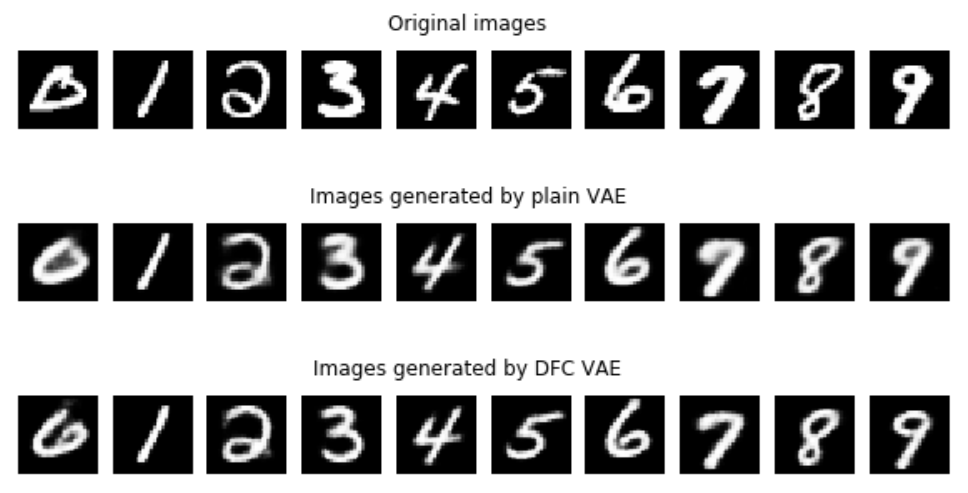
\includegraphics[width=0.8\textwidth]{images/vae_dfc_gen}
    \caption{}
    \label{fig:vae_dfc_recon}
\end{figure}

Na rysunku \ref{fig:dfc_mnist_compare} przedstawiony jest efekt przeprowadzenia analogicznego eksperymentu z nauką na jedynie przykładach z klas [4, 7] i sprawdzeniu zachowania dla danych z klasy 5. Zamiast kosztu rekonstrukcji MSE używamy błędu perceptualnego. Jak widać separacja jest co najmniej tak dobra jak w przypadku zwykłego VAE.

\begin{figure}[h!]
    \centering
    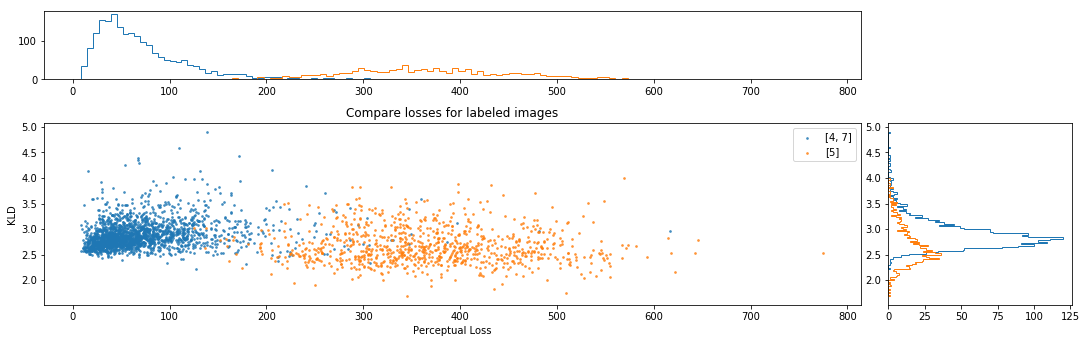
\includegraphics[width=1.0\textwidth]{images/dfc_mnist_compare}
    \caption{}
    \label{fig:dfc_mnist_compare}
\end{figure}
